\chapter{Conceptual Design}
\label{chap:05_design}

In this chapter the conceptual design of the implementation is introduced. The concept in this chapter is based on the theory of \Chap{chap:02_foundation} and uses the technologies introduced in \Chap{chap:04_background}.


% ===========================================
% ===========================================
\section{Choice of Technologies}
\label{sec:05_restrictions}
The following technologies are used to create the conceptual design of the implementation:

\begin{itemize}
% python
\item Python programming language: Python is used as the main programming language for Apache Spark applications.

% docker
\item Docker: Docker is used to deploy components in the computing environment as a container. This enables to create homogeneous nodes in the environment. Furthermore, Docker Swarm is used as orchestration tool and takes care of the health status of each component.

% Gitlab
\item GitLab: The source code repository is hosted on the GitLab platform. Furthermore, the automated deployment pipeline is design using the CI/CD feature of GitLab. Therefore, using GitLab fulfils the version control, and build server requirements mentioned in \Sec{sec:02_depl-pipeline_requirements}.

% Spark
\item Apache Spark: Apache Spark is used to distribute the workload of training machine learning applications across multiple workers. The goal is to scale the replicas of Apache Spark workers to increase the performance of the cluster.

% RAPIDS
\item NVIDIA RAPIDS: In addition to scaling Apache Spark worker node replicas, the NVIDIA RAPIDS plugin suite is used to enable GPU acceleration on the Apache Spark cluster. Enabling Apache Spark to leverage GPUs increases the computational power as well.

% Prom
\item Prometheus: 
Prometheus fulfils all requirements of a monitoring system introduced in \Sec{sec:02_monitoring}. It provides a powerful multi-dimensional data-model and a query language for aggregations and filtering of multi-dimensional time-series data. Additionally, Prometheus is a pull-based monitoring system and includes a time-series database.

% cAdvisor
\item cAdvisor:
cAdvisor serves as a monitoring agent. It scrapes performance metrics from Docker container. Prometheus is able to pull the data from cAdvisor to save it in its time-series database.

% dcgm-exporter
\item dcgm-exporter:
The dcgm-exporter is used as a monitoring agent as well. It is used to monitor the utilization of the available GPUs.
\end{itemize}


% ===========================================
% ===========================================
\section{Identification of Suitable Metrics for Scaling}
\label{sec:05_metrics}
% SHort intro
Suitable metrics are needed to measure the system performance while the Apache Spark cluster is actively performing work.
% Rapids enabled GPU
With the RAPIDS accelerator for Apache Spark, the cluster is able to utilize the computing power of GPUs and CPUs to enable parallization.
% SO?
Therefore, suitable metrics to measure the system performance are the CPU utilization and the GPU utilization during the time when the cluster is actively performing computations.


\subsection{CPU Utilization}
% Sharing CPU cores
All Apache Spark worker run on the same machine. Therefore, all available CPU cores on the machine will be shared across each Apache Spark worker.
%
To get a value that indicates the CPU utilization between 0\% and 100\%, a metric is needed that represents the percentage of time, all performing applications occupy CPU cycles.
% cadvisor
cAdvisor provides a performance metric called \texttt{container\_cpu\_usage\_seconds\_total}\footnote{Monitoring cAdvisor with Prometheus - \url{https://github.com/google/cadvisor/blob/master/docs/storage/prometheus.md} (Accessed: 2021-01-21)}. This metric provides the total amount of CPU seconds consumed by core of a container. 
% Overall utilization
To calculate the overall CPU utilization for all Apache Spark worker, the value of the performance metric for each worker container over a specific rate is summed up.
%
In this case, the CPU utilization ($U_{CPU}$) is defined by \Eq{eq:05_metrics_cpu} with $n \in \mathbb{N} \text{the number of ActiveWorkers}$.

\begin{equation}
U_{CPU}=\sum_{n=1}^{ActiveWorker}container\_cpu\_usage\_seconds\_total_{n}
\label{eq:05_metrics_cpu}
\end{equation}

\subsection{GPU Utilization}
%
In addition to the CPU utilization, Apache Spark worker are able to utilize GPUs to accelerate the computation work.	
% The metric
The dcgm\_exporter agent provides the \texttt{dcgm\_fi\_dev\_gpu\_util} performance metric. This metric returns the procentual utilization per GPU.
% How to calculate
Therefore, the overall GPU utilization ($U_{GPU}$) is defined by \Eq{eq:05_metrics_gpu}.


\begin{equation}
U_{GPU} = \dfrac{\sum dcgm\_fi\_dev\_gpu\_util}{ActiveGPUs}
\label{eq:05_metrics_gpu}
\end{equation}


% ===========================================
% ===========================================
\section{Computing Environment Architecture}
% Single machine
The computing environment will be deployed on a single machine.
% Autonomic
The goal is to create a self-optimizing autonomic computing environment (described in \Sec{sec:02_ac}).
% manage
Furthermore, to manage the components and resources in the environment, an autonomic manager designed according to the MAPE architecture (introduced in \Sec{subsec:02_ac_manager}).
% Docker
For simplicity, each node in the computing environment is deployed as a Docker service in a Docker swarm (introduced in \Sec{subsec:04_docker_swarm}).
% swarm
This allows to define the state of each service which includes the number of replicas. The number of replicas can be updated during runtime.


% Overall design
\begin{figure}[h]
\centering
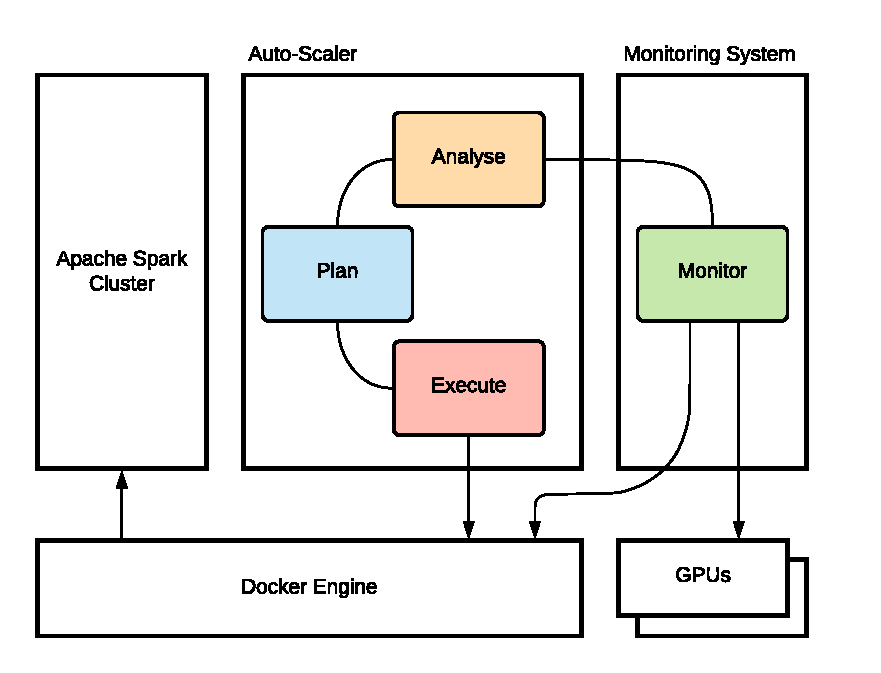
\includegraphics[scale=1]{images/05_conceptual_design/autonomic_manager/control_loop}
\caption{Full MAPE control loop architecture}
\label{fig:05_am_monitoring_loop_arch}
\end{figure}
% Explain 
\Fig{fig:05_am_monitoring_loop_arch} provides an overview over the computing environment concept.
% resources
The managed resources (introduced \Sec{subsec:02_ac_resources}) in this environment are the Apache Spark cluster, and the GPUs.
% manager
These resources are managed by the autonomic manager which consists of the \textit{Auto-Scaler}, and the monitoring system. Furthermore, the autonomic manager implements all four phases of the MAPE architecture and therefore, executes the control-loop.
% Docker 
As being mentioned previously, all components are deployed using Docker. Therefore, to manage components in the computing environment, the autonomic manager needs to interact with the host machines Docker engine.


\paragraph{Control-loop workflow:}
% Workflow figure
\begin{figure}[h]
\centering
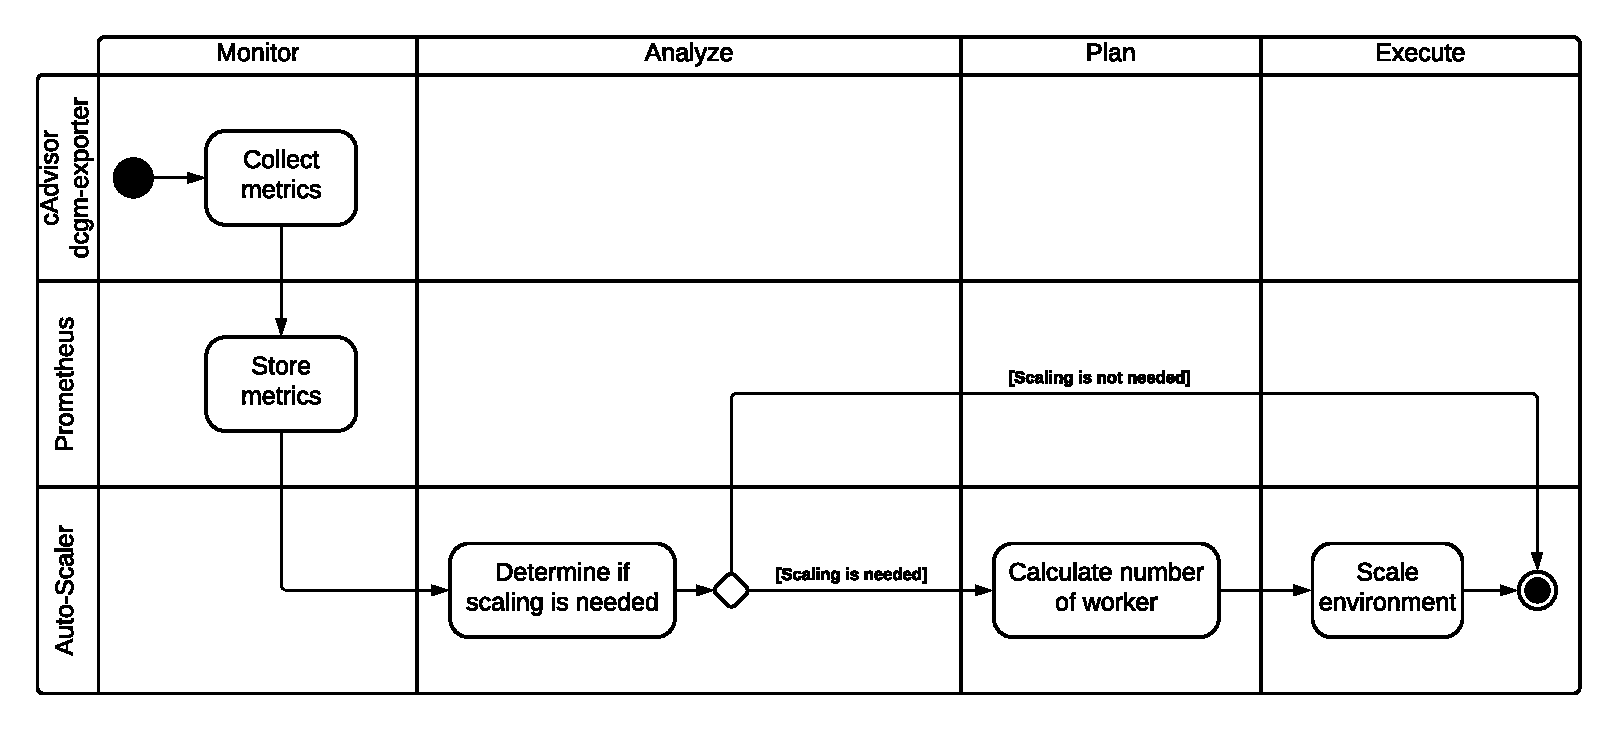
\includegraphics[scale=0.50]{images/05_conceptual_design/autonomic_manager/autonomic_manager_workflow}
\caption{UML activity model of the autonomic manager process}
\label{fig:05_am_monitoring_loop_workflow}
\end{figure}
% Explain
The control-loop workflow is illustrated in \Fig{fig:05_am_monitoring_loop_workflow}.
% Monitor
It starts in the Monitor phase. All monitoring agents (cAdvisor and dcgm-exporter) collect performance metrics from their targets. Next, Prometheus pulls the metrics from all monitoring agents and saves the data in its time-series database.
% Analyze
In the analyse phase, the \textit{Auto-Scaler} determines if a scaling action is necessary. If a scaling action is not needed, the iteration ends.
% Plan
Otherwise, if a scaling action is needed, the \textit{Auto-Scaler} determines the number of Apache Spark worker replicas in the Plan phase.
% Execute
Lastly, in the Execute phase, the \textit{Auto-Scaler} scales the replicas of the Apache Spark worker Docker service.


% ===========================================
% ===========================================
\section{Apache Spark Cluster}
\label{sec:05_spark}
% Short intro
The Apache Spark cluster is the computing unit of the computing environment. It is responsible to distribute the workload of training machine learning models.
% Figure
\begin{figure}[h]
\centering
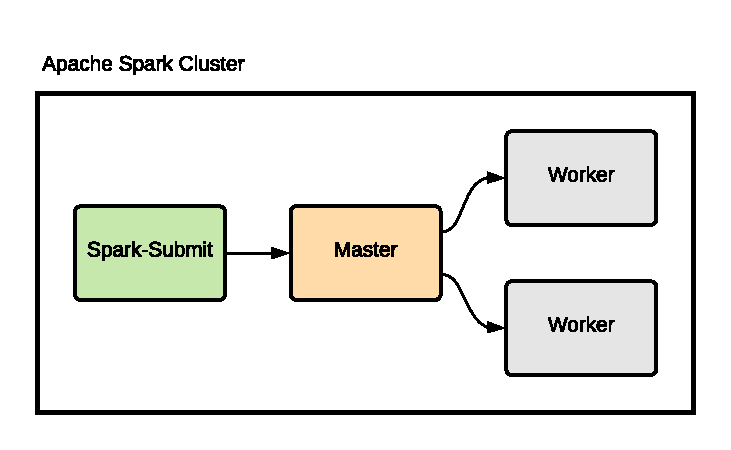
\includegraphics[scale=1]{images/05_conceptual_design/apache_spark/apache_spark_cluster}
\caption{Apache Spark cluster architecture}
\label{fig:05_spark_arch}
\end{figure}
% FIgure intro
In \Fig{fig:05_spark_arch} illustrates the architecture of the Apache Spark cluster. It consists of a master node, multiple worker nodes, and spark-submit nodes.

\begin{itemize}
% Master
\item Master: The master is responsible to distribute the workload of an application, submitted by a \textit{spark-submit} node, across all available worker nodes. The Apache Spark application architecture is explained in \Sec{subsec:04_spark_architecture}.

% Worker
\item Worker: A worker node is responsible to perform the workload given by the master node. Furthermore, the replicas of active worker nodes in the cluster are dynamically adapted by the \textit{Auto-Scaler} at runtime.

\item Spark-Submit: A \textit{spark-submit} node is deployed whenever an application is submitted to the cluster.
\end{itemize}
% Standalone mode
The cluster is deployed in standalone mode (\Sec{subsec:04_spark_standalone}). Because Docker Swarm is used as the orchestration tool which controls the state of nodes, there is no need to use another orchestration tool like Apache Mesos or Kubernetes as cluster manager.
% Docker
Additionally, this simple approach allows to run each node of the cluster in a Docker container without the need of additional configuration.


\subsection{Homogeneous Apache Spark Worker Nodes}
% Short intro
The \textit{Auto-Scaler} scales the replicas of Apache Spark worker nodes. Therefore, the cluster is scaled horizontally. As being explained in \Sec{subsec:02_foundations_scalability_horizontal-scaling}, the horizontal scaling approach is more efficient when scaling homogeneous nodes, because each node adds the same amount of computational power to the cluster cluster.
% How to achieve
To ensure that the worker nodes are homogeneous, the worker Docker service uses the same Docker image for each worker node. The Docker image is created from a custom Dockerfile.
% Resources
This guarantees that each worker uses the same software and has the same amount of computational resources available as each other worker.
% RAPIDS
Additionally, all requirements mentioned in \Sec{subsec:04_rapids_req} to enable GPU acceleration with RAPIDS are installed in a worker image.


\subsection{Deploying an Application with spark-submit}
\label{subsec:05_spark_spark-submit}
% Intro
Whenever the CI pipeline submits an application to the Apache Spark cluster, it deploys a \textit{spark-submit} Docker container to the cluster.
% spark-submit purpose
The purpose of the \textit{spark-submit} container is to submit an application with the spark-submit executable (described in \Sec{subsubsec:04_spark_standalone_submit}) to the cluster.
% No support for python in cluster mode
A standalone mode Apache Spark cluster does not support to submit a Python application with the spark-submit executable from outside of the cluster. Therefore, the spark-submit executable has to be executed on the host machine with access to the master node \cite{Apache2020Spark}.
% Swarm
To submit an application to the master node, the \textit{spark-submit} container needs to be in the same Docker swarm network. The node is deployed as a Docker container instead of a Docker service. Each \textit{spark-submit} container is deployed with a different setting depending on the configuration and application from the CI pipeline. This configuration can be set in the CI pipeline configuration, explained in SEC
% End
After the application has been submitted, the spark-submit node automatically exits.
% Resources
Additionally, the \textit{spark-submit} container sets the amount of resources for the executors running on the worker nodes.


\section{Autonomic Manager}
\label{05_am}
% SHort intro
The autonomic manager is one of the main modules of the computing environment.
% Responsibilites
It is responsible to monitor the performance metrics of all Apache Spark worker nodes and automatically scale the number of worker nodes to adapt to a specified performance goal.
% MAPE
The autonomic manager will be implemented according to the MAPE architecture as described in \Sec{subsec:02_ac_manager}. To create a complete control-loop, the autonomic manager is composed of multiple components as illustrated in \Fig{fig:05_am_concept}.
% A figure explaining the concept
\label{subsec:05_am}
\begin{figure}[h]
\centering
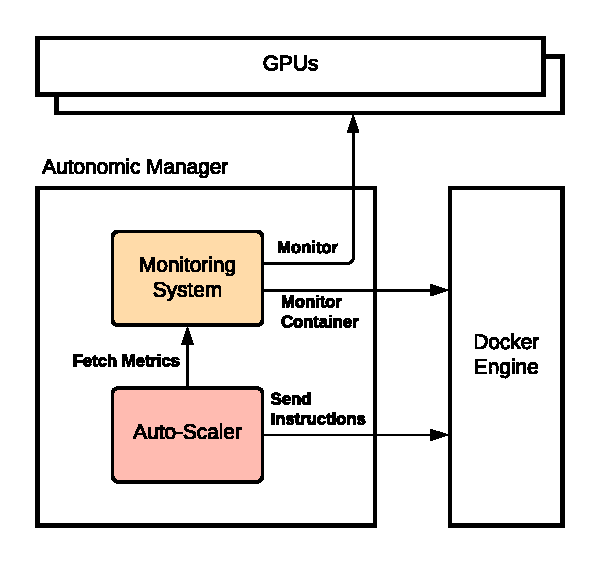
\includegraphics[scale=1]{images/05_conceptual_design/autonomic_manager/autonomic_manager_concept}
\caption{Autonomic manager component design}
\label{fig:05_am_concept}
\end{figure}
% Explain figure
It consists of a monitoring system (theory is explained in \Sec{sec:02_monitoring}) and an \textit{Auto-Scaler} module.
% Docker
Each component in the computing environment is deployed as a Docker service. Therefore, Docker swarm takes care of the health status of each component.
% Monitor
To monitor the performance of Docker container in the computing environment, the autonomic manager needs access to the Docker engine. Additionally, to monitor GPU performance as well, a monitoring agent is needed which is capable of scraping metrics from the GPUs.
% Scaling
Furthermore, the autonomic manager is responsible to scale the replicas of Apache Spark worker nodes. As being introduced in \Sec{sec:05_spark}, a worker service takes care of all worker nodes. Therefore, the autonomic manager needs access to the Docker engine of the host machine to send scaling instructions.


\subsection{Monitoring System}
% Short intro
The monitoring system is responsible to perform the Monitor phase. Therefore it monitors the performance of components in the computing environment and makes them available for the \textit{Auto-Scaler}.
% Responsibilites
In this environment, the monitoring system collects the performance metrics of the Apache Spark worker Docker container and the GPU performance. It is important to mention that the number of worker nodes varies over time because the \textit{Auto-Scaler} scales the replicas of worker nodes according to the system performance.
% The figure
\begin{figure}[h]
\centering
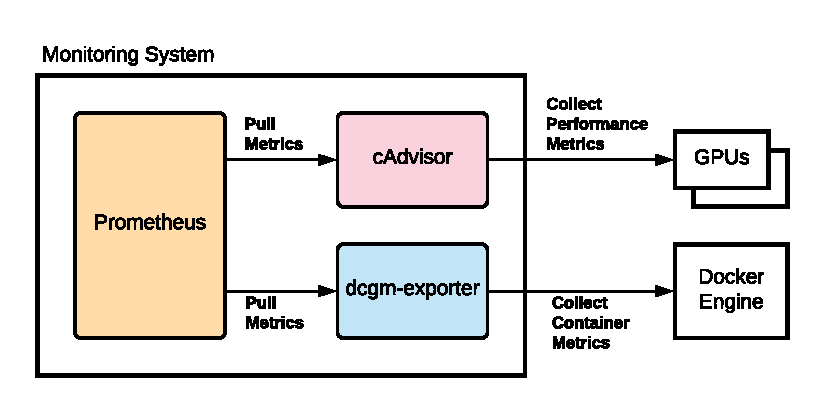
\includegraphics[scale=1]{images/05_conceptual_design/autonomic_manager/monitoring_system_concept}
\caption{Monitoring system conceptual design}
\label{fig:05_am_monitoring_concept}
\end{figure}
% Explain figure
\Fig{fig:05_am_monitoring_concept} illustrates the architecture of the monitoring system. It consists of three components:
% The components
\begin{itemize}
\item dcgm-exporter: A monitoring agent which is responsible to collect GPU performance metrics.
\item cAdvisor: cAdvisor is monitoring agent which collects performance metrics of Docker container in the environment.
\item Prometheus: Prometheus collects the performance metrics from all monitoring agents and saves them as time-series data in a time-series database.
\end{itemize}


\subsection{Auto-Scaler}
% Short intro
The \textit{Auto-Scaler} is the second module of the autonomic manager and responsible to dynamically adjust the replicas of Apache Spark worker nodes in the computing environment to accommodate specified performance goals. 
% MAPE
It implements the Analyse, Plan, and Execute phases of the MAPE architecture. Together with the monitoring system, it creates a complete autonomic manager implementing all phases of the MAPE architecture.
% Reactive threshold based 
The \textit{Auto-Scaler} is designed as a reactive auto-scaler and uses a threshold-based algorithm to adapt the number of worker nodes. To define the thresholds, it can be configured using a configuration file.


% Prom API
As illustrated in \Fig{fig:05_am_concept}, the \textit{Auto-Scaler} fetches performance metrics from the monitoring system via the Prometheus HTTP API.
% Phases
After it received the performance metrics, the \textit{Auto-Scaler} analyses the metrics, plans scaling-actions to adjust the number of worker replicas and sends instructions to the Docker engine.


\subsubsection{MAPE Phases}
% SHort intro
As being mentioned, the \textit{Auto-Scaler} implements the Analyse, Plan, and Execute phases of the MAPE architecture. Each phase has a different workflow to accommodate its goal.

\paragraph{Analyse:}
% How to analyze
During each period, the \textit{Auto-Scaler} fetches the performance metrics defined in the configuration from the Prometheus HTTP API.
% Determine if scaling is needed
After the metrics are received, the \textit{Auto-Scaler} determines if a scaling action is needed using the Scaling Heat algorithm (introduced in \Sec{sec:04_background_scaling-heat}). If scaling is not necessary, the \textit{Auto-Scaler} continues to collect and analyse performance metrics.

\paragraph{Plan:}
% Short intro
If a scaling-action is necessary, the \textit{Auto-Scaler} is responsible to determine the number of Apache Spark worker replicas, needed to reach the defined utilization goal.
% Calculating Spark worker
To calculate the number of worker nodes, the \textit{Auto-Scaler} uses the Kubernetes Horizontal Pod Auto-Scaling algorithm (introduced in \Sec{sec:04_background_khpa}).
% Thresholds
It is possible, that the number of needed replicas violates the upper or lower thresholds of active Apache Spark worker nodes. Then, the Auto-Scaler uses the maximum or minimum number of worker nodes as the desired replicas.

\paragraph{Execute:}
% Short intro
After the number of needed replicas have been calculated, the \textit{Auto-Scaler} sends the instruction to scale the Apache Spark worker service to the desired number of replicas.
% Cooldown
Afterwards, a cooldown period gets activated. This brings the effect, that the Apache Spark cluster needs time to distribute the workload across all new worker nodes efficiently. During the cooldown period, no scaling actions are executed.


\subsubsection{Configuration}
\label{subsubsec:05_am_auto-scaler_config}
The \textit{Auto-Scaler} needs specific configuration properties to be able to collect the correct metrics from Prometheus and scale the Apache Spark worker service replicas. The following are properties that have to be defined to ensure that the \textit{Auto-Scaler} is able to collect meaningful metrics and scale Apache Spark worker as expected.

\begin{itemize}
\item General properties:
\begin{itemize}
\item Interval seconds: The number of seconds after the \textit{Auto-Scaler} starts a new process.

\item Cooldown period: The duration in seconds,  the \textit{Auto-Scaler} has to wait after a scaling action was performed.

\item Recurrence factor: To prevent to many scaling actions,  the autonomic manager should only execute a scaling action,  if the utilization thresholds is violated $n$ times.

\item Prometheus URL: The URL of the Prometheus HTTP API.
\end{itemize}

\item Metrics:
To analyse multiple metrics, the user should be able to create a list of metrics. Each metric needs to have a variety of properties configured.
\begin{itemize}
\item Target utilization: The target utilization of a performance metric is needed by the KHPA algorithm to calculate the number of desired replicas.

\item Utilization thresholds: To determine if a scaling action is needed, the scaling heat algorithm needs the minimum and maximum utilization of the performance metric. This value is used by the Scaling-Heat algorithm.

\item Query: A PromQL query defines a performance metric.
\end{itemize}

\item Apache Spark worker properties:
\begin{itemize}
\item Worker service name: The name of the worker Docker service is needed to update the number of replicas.

\item Worker thresholds: The minimum and maximum number of concurrent Spark worker should be defined. To avoid the cold start effect, the minimum amount of worker should be at least 1. 

\item Apache Spark master URI: To distribute the workload across all Spark Worker, all Spark Worker need to communicate with the Spark master.
\end{itemize}
\end{itemize}


% ===========================================
% ===========================================
\section{Automated Deployment Pipeline}
\label{sec:05_pipeline}
% Abstract
An objective of this thesis is to train Machine Learning models, by automatically submitting Apache Spark applications to an Apache Spark cluster. Therefore, the training process of a model has to be integrated into the applications development lifecycle.
%
The applications development lifecycle is automated using the concept of a deployment pipeline (introduced in \Sec{sec:02_depl-pipeline}).
%
In this conceptual design, a CI pipeline is demonstrated which automates the training phase of an application and additionally submits the application to an Apache Spark cluster after the testing was successful.


% Conceptual figure
\begin{figure}[h]
\centering
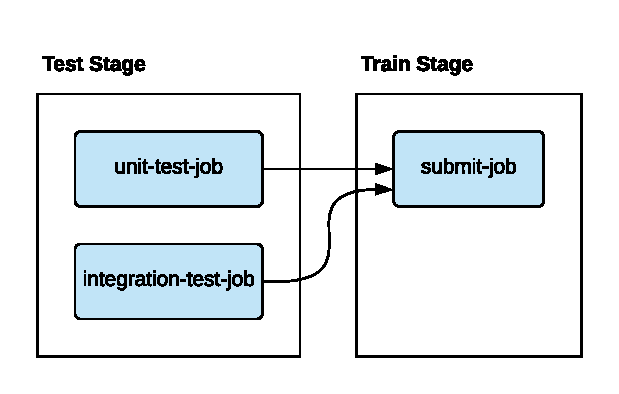
\includegraphics[scale=1]{images/05_conceptual_design/automated_deployment_pipeline/ci_cd_concept}
\caption{Automated Deployment Pipeline concept}
\label{fig:05_deployment_concept}
\end{figure}
% Short intro
\Fig{fig:05_deployment_concept} illustrates the conceptual design of the CI pipeline which consists of two stages:
\begin{enumerate}
\item Test stage: Responsible to perform all tests to validate the applications source code.
\item Train stage: If the test stage has been successful, the application is submitted to the Apache Spark cluster to train the model.
\end{enumerate}
% No build stage
It is important to mention, that a build stage is missing in this conceptual design. The build stage includes compiling source code into a format that can be executed directly.
% Python
Python is an interpreted language and does not need to be compiled for execution.


\subsection{Test Stage}
% short intro
Before the training the machine learning model, the applications source has to be validated by a series of tests.
% responsibilities
Tests can include:
% Tests
\begin{itemize}
\item Unit tests
\item Integration tests
\item End-to-end tests
\end{itemize}
% Different jobs
Each test is being performed in its own job. All jobs perform in parallel after the test stage has been triggered.
% On failure
If a job fails, the whole test stage is marked as failure and all participating developers will get a notification.


\subsection{Train Stage}
\paragraph{}
% Short intro
The train stage is responsible to submit the Apache Spark application to the Apache cluster after the test state was successful.
% How
To submit an application to the Apache Spark cluster, a \textit{spark-submit} Docker container has to be deployed to the same Docker network. How a spark-submit container performs an application is explained in \Sec{subsec:05_spark_spark-submit}.

\paragraph{}
% Same machine with runner
Deploying \textit{spark-submit} Docker container in the Apache Spark cluster network requires access to the overlying Docker engine.
To access the Docker engine within a job of the train stage, the job has to be executed by a GitLab runner on the same host machine.
% Perform train stage concept
\begin{figure}[h]
\centering
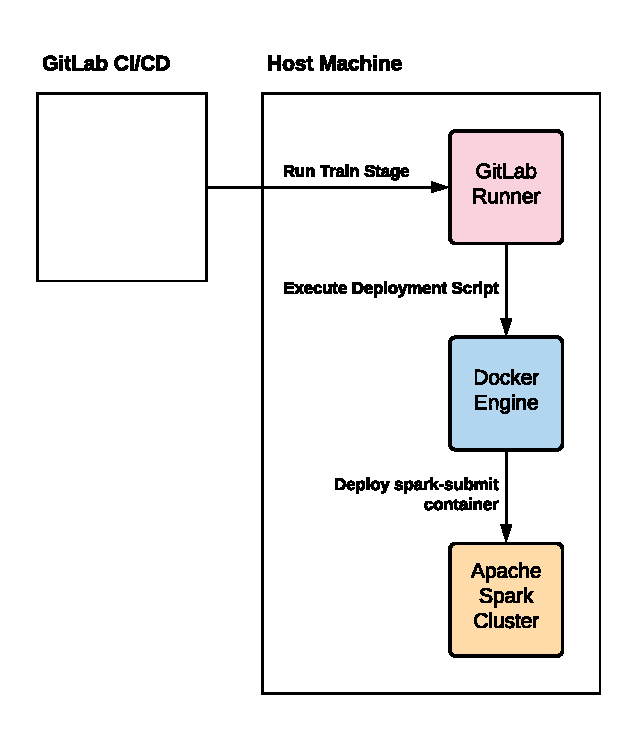
\includegraphics[scale=1]{images/05_conceptual_design/automated_deployment_pipeline/train_stage_runner}
\caption{Deployment of a spark-submit container}
\label{fig:05_deployment_train_concept}
\end{figure}
% Explain figure
\Fig{fig:05_deployment_train_concept} illustrates the steps to deploy a \textit{spark-submit} container in the Apache Spark cluster swarm network.
% Runner
The GitLab CI/CD server connects to a GitLab on the host machine and instructs it to execute the train stage.
Then, the runner performs the scripts whicn instruct the Docker engine to deploy a spark-submit container in the Apache Spark cluster.
